%-------------------------------------------------------------------------------
% This file provides a skeleton ATLAS note.
% \pdfinclusioncopyfonts=1
% This command may be needed in order to get \ell in PDF plots to appear. Found in
% https://tex.stackexchange.com/questions/322010/pdflatex-glyph-undefined-symbols-disappear-from-included-pdf
%-------------------------------------------------------------------------------
% Specify where ATLAS LaTeX style files can be found.
\RequirePackage{latex/atlaslatexpath}
% Comment out the above line if the files are in a central location, e.g. $HOME/texmf.
%-------------------------------------------------------------------------------
\documentclass[NOTE, atlasdraft=true, texlive=2019, UKenglish]{atlasdoc}
% The language of the document must be set: usually UKenglish or USenglish.
% british and american also work!
% Commonly used options:
%  atlasdraft=true|false This document is an ATLAS draft.
%  texlive=YYYY          Specify TeX Live version (2016 is default).
%  coverpage             Create ATLAS draft cover page for collaboration circulation.
%                        See atlas-draft-cover.tex for a list of variables that should be defined.
%  cernpreprint          Create front page for a CERN preprint.
%                        See atlas-preprint-cover.tex for a list of variables that should be defined.
%  NOTE                  The document is an ATLAS note (draft).
%  PAPER                 The document is an ATLAS paper (draft).
%  CONF                  The document is a CONF note (draft).
%  PUB                   The document is a PUB note (draft).
%  BOOK                  The document is of book form, like an LOI or TDR (draft)
%  txfonts=true|false    Use txfonts rather than the default newtx
%  paper=a4|letter       Set paper size to A4 (default) or letter.

%-------------------------------------------------------------------------------
% Extra packages:
\usepackage{atlaspackage}
% Commonly used options:
%  biblatex=true|false   Use biblatex (default) or bibtex for the bibliography.
%  backend=bibtex        Use the bibtex backend rather than biber.
%  subfigure|subfig|subcaption  to use one of these packages for figures in figures.
%  minimal               Minimal set of packages.
%  default               Standard set of packages.
%  full                  Full set of packages.
%-------------------------------------------------------------------------------
% Style file with biblatex options for ATLAS documents.
\usepackage{atlasbiblatex}
\usepackage{colortbl}
\usepackage{float}
\restylefloat{table}
% Commonly used options:
%  backref=true|false    Turn on or off back references in the bibliography.

% Package for creating list of authors and contributors to the analysis.
\usepackage{atlascontribute}

% Useful macros
\usepackage[process=true]{atlasphysics}
% See doc/atlas_physics.pdf for a list of the defined symbols.
% Default options are:
%   true:  journal, misc, particle, unit, xref
%   false: BSM, heppparticle, hepprocess, hion, jetetmiss, math, process,
%          other, snippets, texmf
% See the package for details on the options.

% Macro to add to-do notes (for several authors). Uses the todonotes package.
% \ATLnote{JS}{Jane}{green!20}{green!50!black!60}
% add macros \JSnote and \JSinote for notes in the margin and inline.
% Set output=false in order not to print out the notes.
% Comment this out for the final version of the note.
\usepackage[output=true]{atlastodo}


% Files with references for use with biblatex.
% Note that biber gives an error if it finds empty bib files.
\addbibresource{QTDiego.bib}
\addbibresource{bib/ATLAS.bib}
\addbibresource{bib/CMS.bib}
\addbibresource{bib/ConfNotes.bib}
\addbibresource{bib/PubNotes.bib}

% Paths for figures - do not forget the / at the end of the directory name.
\graphicspath{{logos/}{figures/}}

% Add your own definitions here (file QTDiego-defs.sty).
\usepackage{QTDiego-defs}

%-------------------------------------------------------------------------------
% Generic document information
%-------------------------------------------------------------------------------

% Title, abstract and document 
%-------------------------------------------------------------------------------
% This file contains the title, author and abstract.
% It also contains all relevant document numbers used for an ATLAS note.
%-------------------------------------------------------------------------------

% Title
\AtlasTitle{Tau-ID Scale Factors for high-$\pt$ taus using boosted $Z\to\tau\tau$ events.}

% Draft version:
% Should be 1.0 for the first circulation, and 2.0 for the second circulation.
% If given, adds draft version on front page, a 'DRAFT' box on top of each other page, 
% and line numbers.
% Comment or remove in final version.
\AtlasVersion{0.1}

% Abstract - % directly after { is important for correct indentation
\AtlasAbstract{%
  Different algorithms have been trained by the ATLAS collaboration to separate true semi-hadronically decaying taus from QCD jets. The efficiency of these algorithms is compared in simulation and data and correction factors are derived to account for the differences that may arise from the simulation limitations. This study aims to evaluate the correction factors for the tau-ID algorithms for high-$\pt$ taus. Highly boosted $Z\to\tauhad\taulep$ events in the transverse plane, where $l=e,\mu$ are used.  The scale factors are calculated as a double ratio between $Z\to\tauhad\taulep$ and $\Zll$ events. This aims to cancel phenomenological and light-lepton related uncertainties. In this report, we present the value obtained for the scale factors for the classifier \textit{tight-ID} working point. The values are $C_{\text{Tight-ID}}=0.989\pm 0.012\text{(stat)}\pm 0.024\text{(lumi)}\pm 0.028\text{(sys)}$ for the muon-tau final state and $C_{\text{Tight-ID}}=0.974\pm 0.014\text{(stat)}\pm 0.023\text{(lumi)}\pm 0.029\text{(sys)}$ for the electron-tau final state.
}

% Author - this does not work with revtex (add it after \begin{document})
\author{The ATLAS Collaboration}

% Authors and list of contributors to the analysis
% \AtlasAuthorContributor also adds the name to the author list
% Include package latex/atlascontribute to use this
% Use authblk package if there are multiple authors, which is included by latex/atlascontribute
% \usepackage{authblk}
% Use the following 3 lines to have all institutes on one line
% \makeatletter
% \renewcommand\AB@affilsepx{, \protect\Affilfont}
% \makeatother
% \renewcommand\Authands{, } % avoid ``. and'' for last author
% \renewcommand\Affilfont{\itshape\small} % affiliation formatting
% \AtlasAuthorContributor{First AtlasAuthorContributor}{a}{Author's contribution.}
% \AtlasAuthorContributor{Second AtlasAuthorContributor}{b}{Author's contribution.}
% \AtlasAuthorContributor{Third AtlasAuthorContributor}{a}{Author's contribution.}
% \AtlasContributor{Fourth AtlasContributor}{Contribution to the analysis.}
 \author[a]{Diego Baron}
 \author[a]{Terry Wyatt}
% \author[b]{Third Author}
 \affil[a]{University of Manchester}
% \affil[b]{Another Institution}

% If a special author list should be indicated via a link use the following code:
% Include the two lines below if you do not use atlasstyle:
% \usepackage[marginal,hang]{footmisc}
% \setlength{\footnotemargin}{0.5em}
% Use the following lines in all cases:
% \usepackage{authblk}
% \author{The ATLAS Collaboration%
% \thanks{The full author list can be found at:\newline
%   \url{https://atlas.web.cern.ch/Atlas/PUBNOTES/ATL-PHYS-PUB-2020-007/authorlist.pdf}}
% }

% ATLAS reference code, to help ATLAS members to locate the paper
\AtlasRefCode{GROUP-2020-XX}

% ATLAS note number. Can be an COM, INT, PUB or CONF note
% \AtlasNote{ATLAS-CONF-2020-XXX}
% \AtlasNote{ATL-PHYS-PUB-2020-XXX}
% \AtlasNote{ATL-COM-PHYS-2020-XXX}

% Author and title for the PDF file
\hypersetup{pdftitle={ATLAS document},pdfauthor={Diego Baron}}

%-------------------------------------------------------------------------------
% Content
%-------------------------------------------------------------------------------
\begin{document}

\maketitle

\tableofcontents

% List of contributors - print here or after the Bibliography.
%\PrintAtlasContribute{0.30}
%\clearpage

% List of to-do notes
% \listoftodos

%-------------------------------------------------------------------------------
\section{Introduction}\label{Intro}
\label{sec:intro}
%-------------------------------------------------------------------------------

The tau lepton has a proper decay length of 87 $\mu$m \cite{PhysRevD.98.030001}. For this reason, tau leptons usually decay before they can reach the innermost layer of the ATLAS detector. Therefore, only the decay products of the tau leptons can be observed. The tau lepton mass of 1.777 GeV makes this particle the only lepton that can decay into hadrons \cite{PhysRevD.98.030001}. Tau decays can be either leptonically ($\tau\to\nu_\tau\nu_l l$, $l=e,\mu$) or semi-hadronically ($\tau\to\nu_\tau+$hadrons), the latter ones are commonly referred simply as hadronic tau decays ($\tauhad$). Muons and electrons from leptonic tau decays do not have enough kinematical features that can make them easily distinguishable from prompt muons or electrons. In the case of $\tauhad$ decays, which represent approximately 65\% of the tau branching fraction, the decay modes include one or three charged pions. Therefore, the signature of these decays are jets with one or three charged tracks, with a charge correlation and being more collimated than jets initiated from quark or gluon radiation.

Algorithms trained to identify true $\tauhad$ and separating them from misidentified $\tauhad$  candidates, originating from QCD processes, have been developed \cite{Deutsch:2680523}. The most novel of these algorithms is a recurrent neural network (RNN) that uses track and calorimeter information in order to classify true and fake $\tauhad$ candidates. The RNN is now used as the default tau identification criteria for the data recorded by the ATLAS experiment from 2015 to 2018 and has been used as well in 2018 tau lepton triggers.

When the efficiency of the RNN algorithm is measured in data and simulation, a correction or scale factor (SF) is derived and then applied to the simulation in order for the signal efficiency to agree between data and simulation. For high-$\pt$ taus, $t\bar{t}$ events are often used to derive the SFs, since the high top quark mass boosts the decays. However, by measuring the SFs in this way one could be correcting for possible new physics coming from lepton universality violation effects in the W boson decays.

This work is aimed to measure the correction factors for tau identification in the high-$\pt$ regime using boosted $Z\to\tauhad\taulep$ events. Since lepton universality has been tested to far better precision in Z decays, our measurement is safe from lepton universality violating effects.

This report is structured as follows. In Chapter \ref{DataMC}, we present the description of the data and simulation samples used in this work. Chapter \ref{Ana}  describes the analysis methodology, the event selection is presented and the definition of the scale factors is given. The background estimation is discussed in Chapter \ref{BG}. In Chapter \ref{Sys}, the systematic uncertainties for our analysis are presented. The results of our analysis and a discussion is in Chapter \ref{Results}. Finally in Chapter \ref{Conclusion}, conclusions and prospects are discussed.



%-------------------------------------------------------------------------------
\section{Data and MC Samples}\label{DataMC}
\label{sec:samples}
%-------------------------------------------------------------------------------

The data used for this study has been recorded during the Run-II of the LHC. It corresponds to the 2015-2018 data taking period, the total integrated luminosity corresponds to 139.2 $\ifb	$ of proton-proton collisions at a centre-of-mass energy of $\sqrt{s}=13$ TeV.

Monte Carlo (MC) samples are used for signal and background process simulation. For $\Zll$ events two MC samples are used, $\POWPY[8]$ and $\SHERPA$. For the background processes we use $\POWPY[8]$, except for the di-boson samples which are simulated with $\SHERPA$. Table \ref{Table3} shows the MC generators used for each process. An additional table with the complete set of samples is presented in appendix \ref{SampleFiles}.

\begin{table}[htbp]
	\centering
	\begin{tabular}{cc}
		\hline
		\multicolumn{1}{|c|}{Process}  & \multicolumn{1}{c|}{Event Generator} \\ \hline
		$Z\to\tau\tau$                 & $\POWPY[8]$ and $\SHERPA$           \\
		$Z\to ee$                      & $\POWPY[8]$ and $\SHERPA$           \\
		$Z\to\mu\mu$                   & $\POWPY[8]$ and $\SHERPA$           \\
		$W\to l\nu_l$				   & $\POWPY[8]$                       \\
		$t\bar{t}$                     & $\POWPY[8]$                       \\
		Single $t$                     & $\POWPY[8]$                       \\
		Diboson                        & $\SHERPA$                       \\ \hline
	\end{tabular}
	\caption{List of MC event generators used.}
	\label{Table3}
\end{table}


%-------------------------------------------------------------------------------
\section{Analysis Strategy}\label{Ana}
\label{sec:analysis}
%-------------------------------------------------------------------------------

This section describes the analysis methodology. We use boosted $Z\to\tauhad\taulep$ events to measure Monte Carlo correction factors for the tau identification algorithms in the high-$\pt$ region.

Different working points are defined for RNN score relative to the efficiency of selecting true $\tauhad$ candidates. When the efficiency of the working points is measured in data and simulation, a correction factor has to be derived and then applied to the simulation in order for the signal efficiency to agree between data and simulation \cite{ATLAS:2017mpa}. Because of the top quark mass, $t\bar{t}$ events are usually used as a source of high momentum taus for measuring correction factors on the high-$p_T$ bins. However, Lepton universality may not hold in W decays. For that reason our study is aimed to use boosted $Z\to\tauhad\taulep$ events for deriving and cross checking the simulation correction factors in the high-$p_T$ region.   
\section{Signal events}\label{signalevents}
For this study, we consider as signal events where one the taus decays hadronically and the other leptonically, either into an electron or a muon. Thus, our final states will include a $\tauhad$ candidate and a lepton $l=e,\mu$. The presence of the light lepton will be used as our tag. 
Generally, in $\Zll$ events, the taus are produced back to back and their $\pt$ spectrum falls sharply. One way to select events where the taus are boosted in the transverse plane is to look for events where the opening angle in the transverse plane between the taus ($\Delta\phi(\tauhad,\taulep)$) is more acute. A depiction of the topologies of our signal events is shown in Fig.\ref{Fig1}. For these events, the missing transverse momentum ($\met$) is assumed to come from the neutrinos produced in the decays of the tau leptons. Due to the fact that two neutrinos are produced in the leptonic decay mode we expect our events to have a larger $\met$ component along the $\taulep$ direction.
\begin{figure}[htbp]
	\centering
	\subfloat[]{\label{Fig1a}{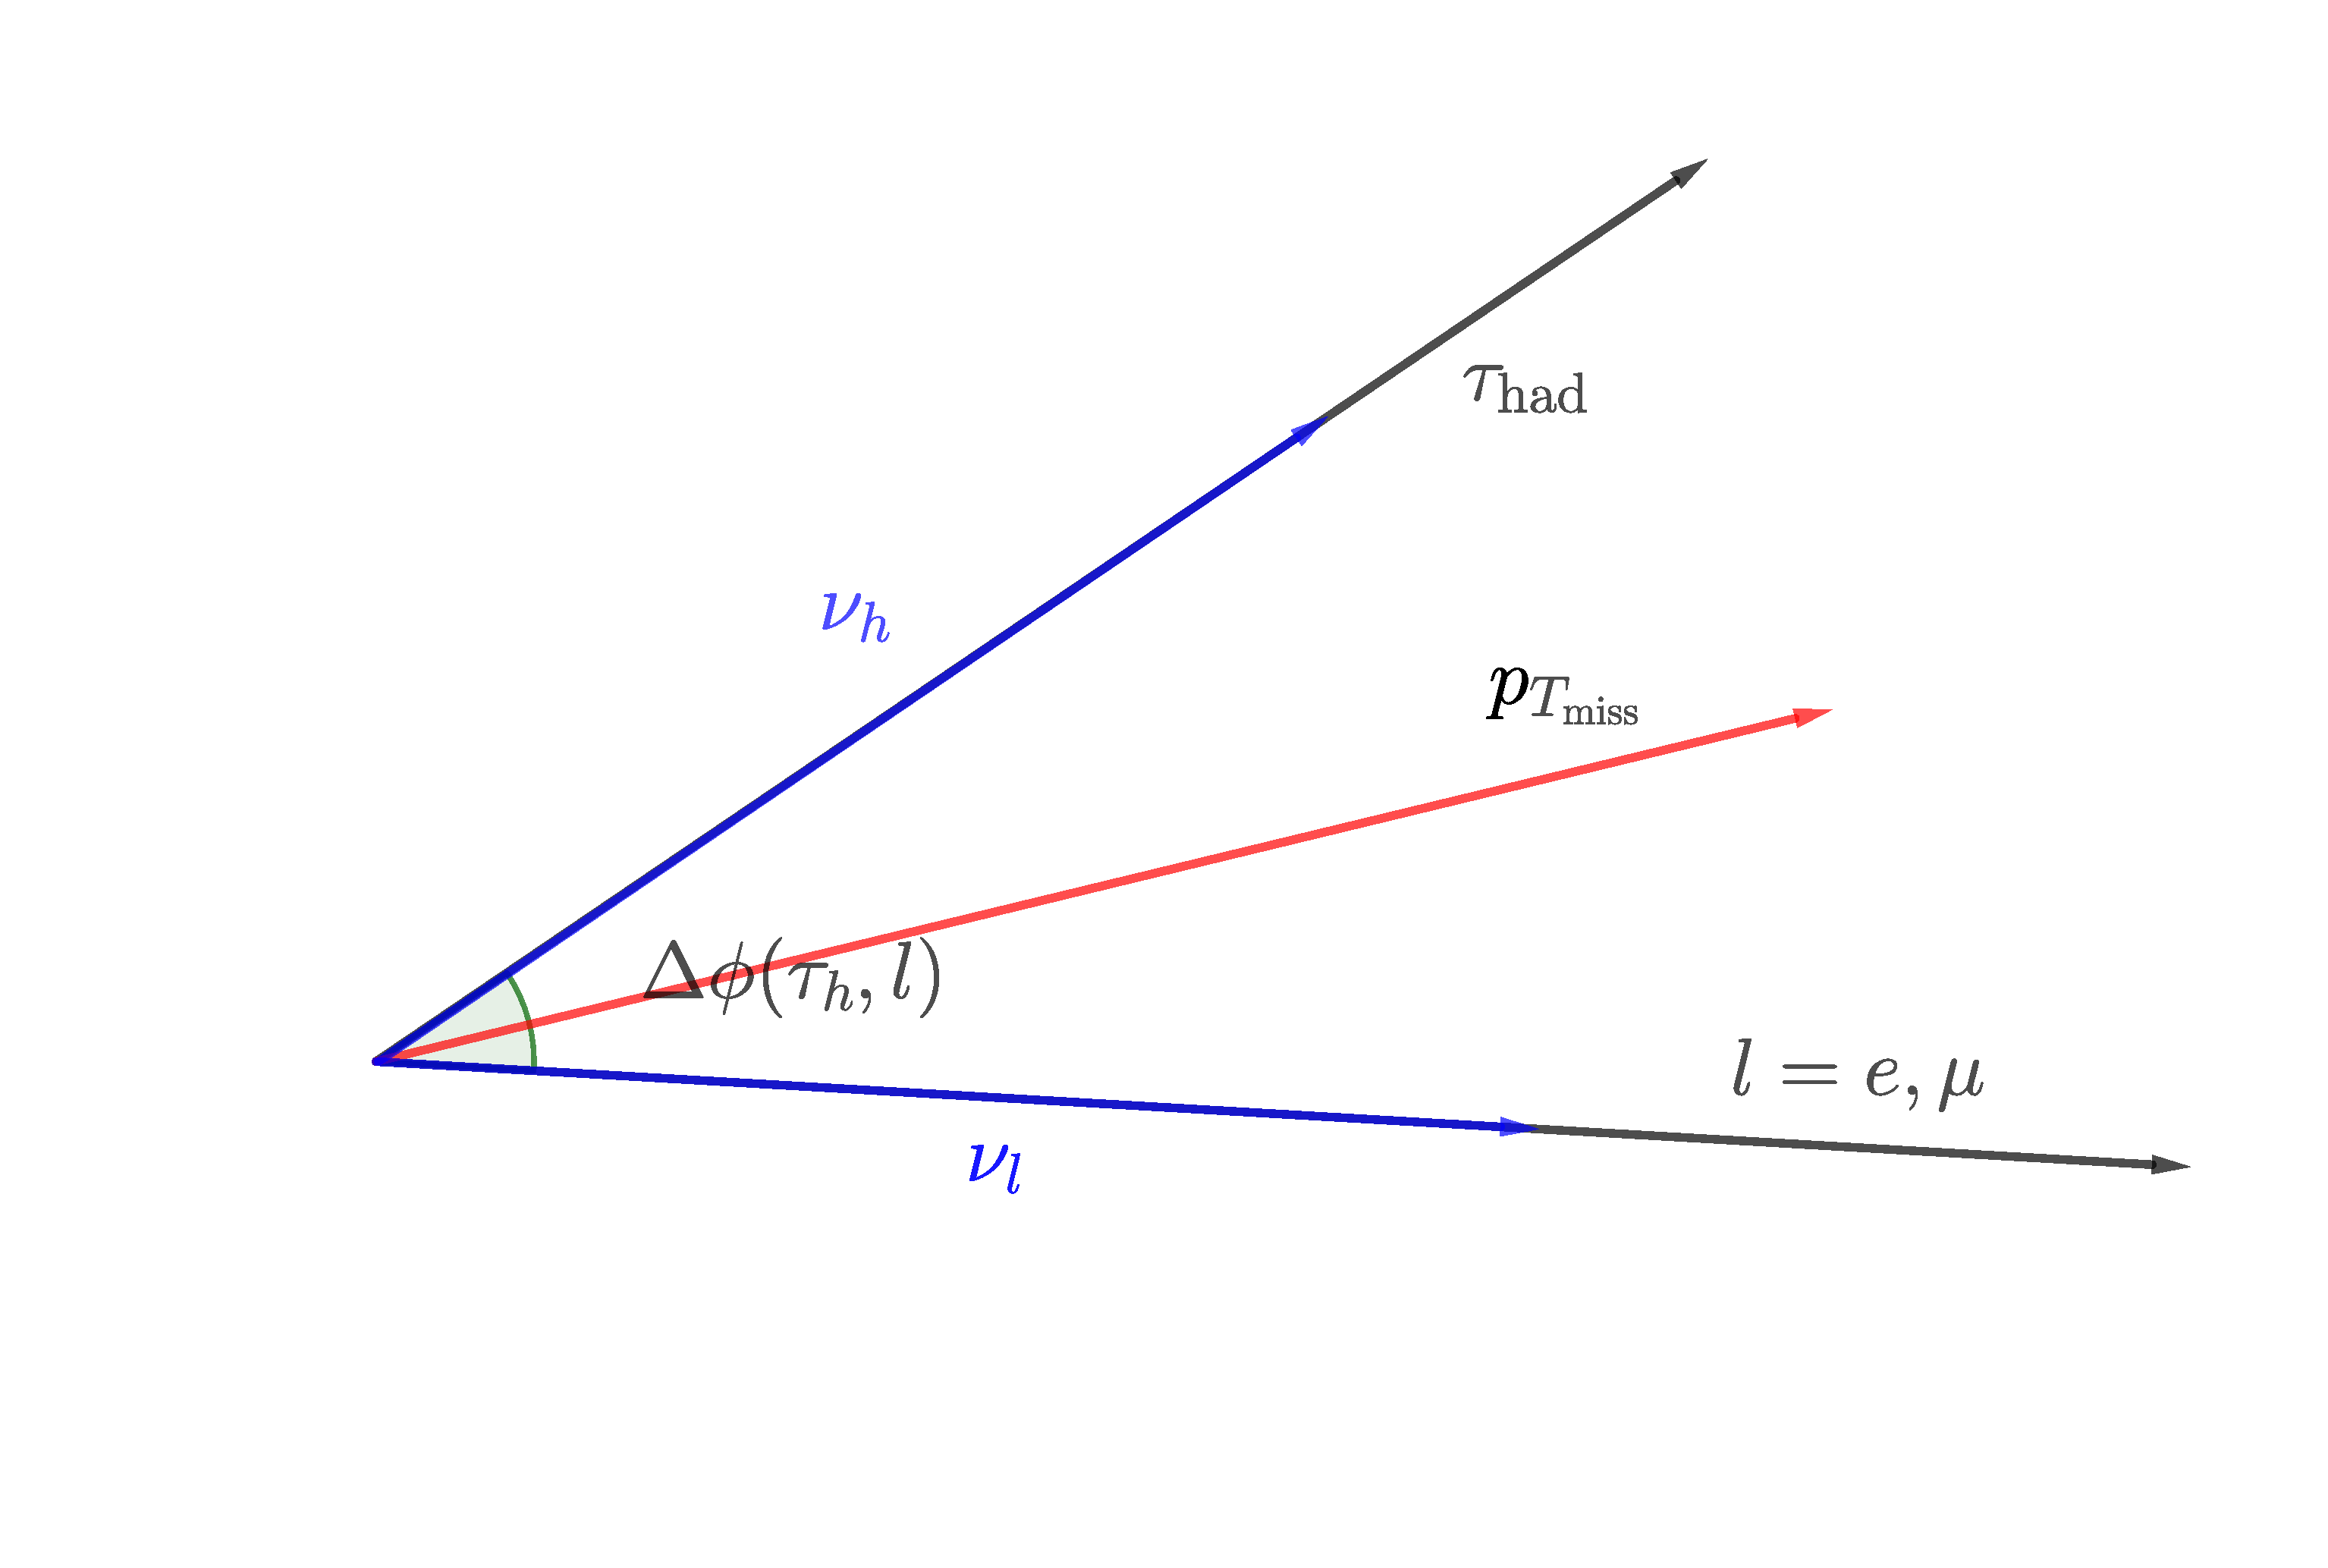
\includegraphics[width=0.49\textwidth]{Fig1a}}}\hfill
	\subfloat[]{\label{Fig1b}{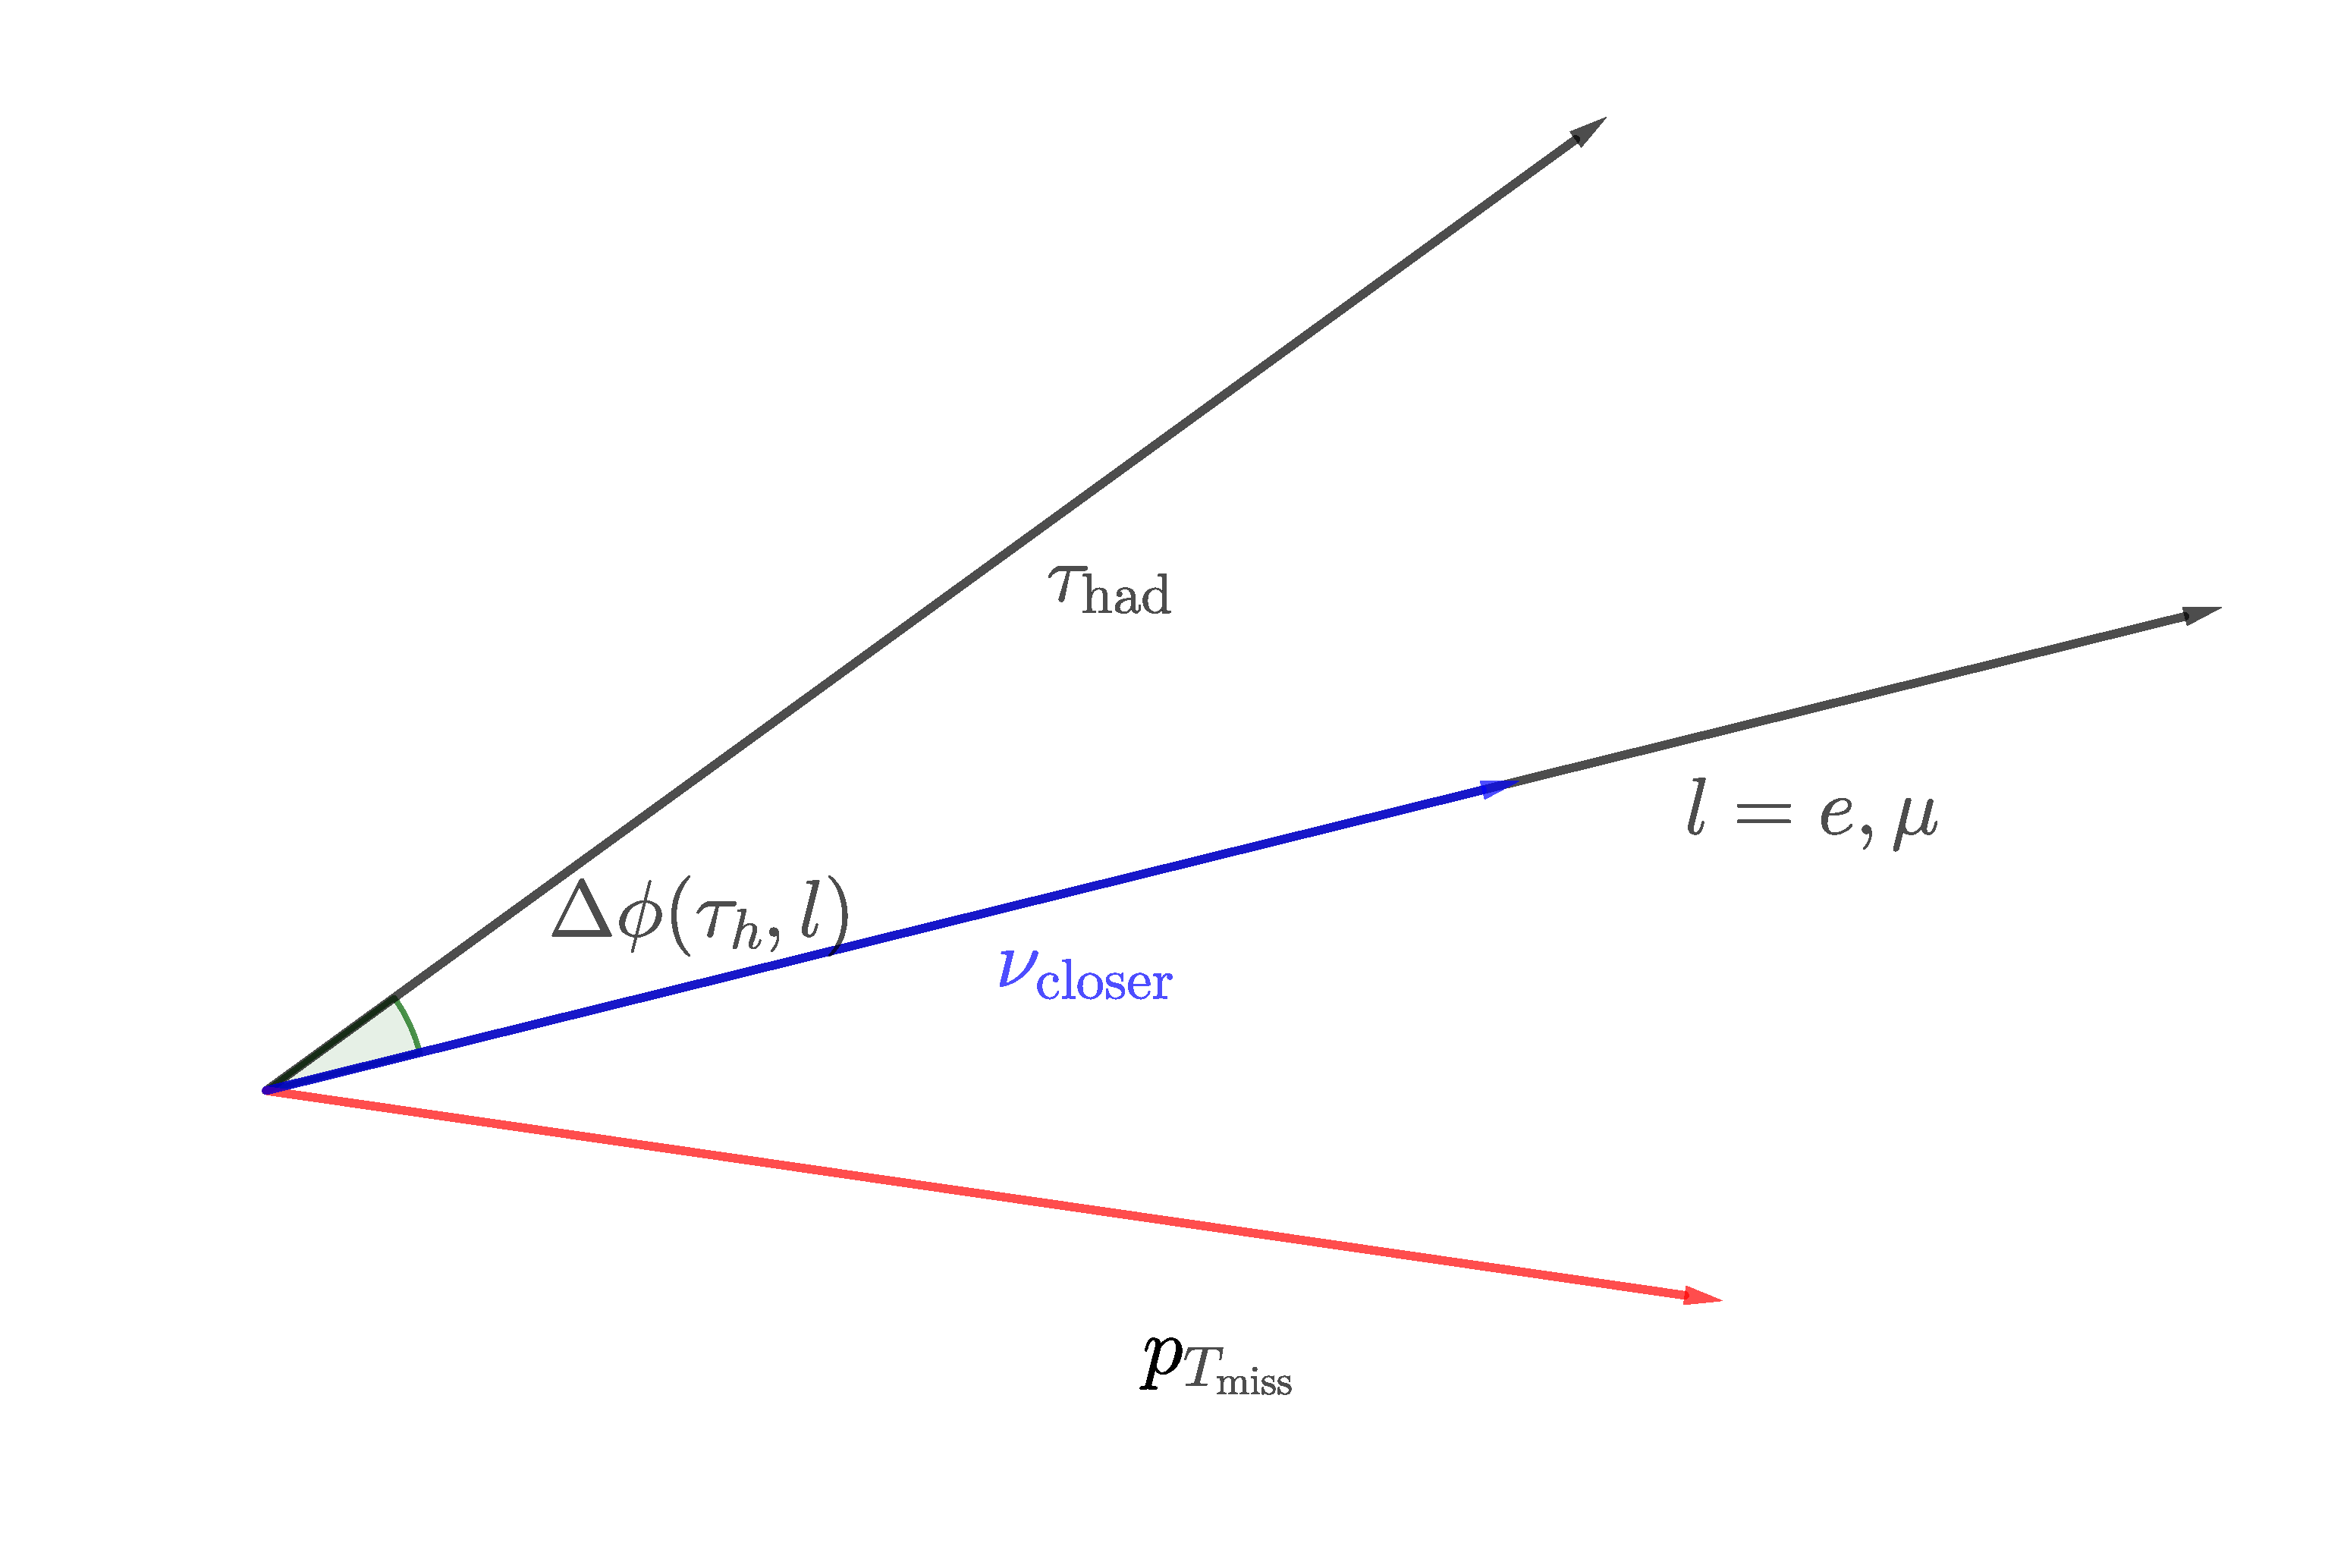
\includegraphics[width=0.49\textwidth]{Fig1b}}}
	\caption{The two different types of topologies that define signal events. On the left, when the missing energy is between the visible objects two neutrinos are assumed to be responsible for all the missing energy. On the right, only one neutrino is assumed to be flying on the direction of the visible object closest to the missing energy.}
	\label{Fig1}
\end{figure}

%-------------------------------------------------------------------------------
\section{Background Estimation}\label{BG}
\label{sec:background}

In the tau reconstruction, $\tauhad$ candidates are seeded from jets. Therefore, QCD events represent the main source of background (BG). Nonetheless, we do not have MC simulations for this processes. For this reason, we use a \textit{data driven method} to estimate multi-jet (MJ). In this section we will discuss how we derived our Multi-Jet Background (MJBG) estimation.

\subsection{Multi-Jet Background}
To obtain the MJBG, a variable that in principle is supposed to be uncorrelated with the shape of the MJBG is chosen. For our study, this variable is the relative sign between the charges of the $\tauhad$ and the lepton. This defines two regions: the same sign (SS) region where $q(\tauhad)=q(l)$ and the opposite sign region where $q(\tauhad)=-q(l)$. Our estimate for the MJBG in the SS region is obtained by subtracting signal and electroweak backgrounds (EWBG) contributions:
\begin{equation}
\text{MJBG}_{\text{SS}}=\text{Data}_{\text{SS}}-\text{Signal}_{\text{SS}}-\text{EWBG}_{\text{SS}},
\label{eq19}
\end{equation}
To study the residual charge correlation, we define a control region (CR) where the MJ background is enhanced. The estimate for the MJBG in these regions is given by eq. \ref{eq19} as well. The region described in Sec.\ref{sec3.3}, which contains all our final selected events is called the signal region (SR). In contrast to the SR, the CR is defined by events that fail the lepton isolation criteria and that fail the Tight-ID working point criterion for the $\tauhad$ candidate. In this region, tau candidates are required to have a looser tau-$pt$ of 25 GeV or more. This last choice was made to increase the number of candidates in the CR. The other kinematic features of the SR are maintained. A diagram showing the four regions just defined is shown in Fig.\ref{Fig7}. Now, if we assume that charge correlation is the same in the SR and CR, we have:
 \begin{equation}
 \frac{\text{MJBG}_{\text{SR OS}}}{\text{MJBG}_{\text{SR SS}}}=\frac{\text{MJBG}_{\text{CR OS}}}{\text{MJBG}_{\text{CR SS}}},
 \end{equation}
then,
 \begin{equation}
\text{MJBG}_{\text{SR OS}}=\text{MJBG}_{\text{SR SS}}\times \text{RQCD}\,
\label{eq36}
\end{equation}
where $\text{RQCD}\equiv\frac{\text{MJBG}_{\text{CR OS}}}{\text{MJBG}_{\text{CR SS}}}$. So, \eqref{eq36} gives the estimation of MJBG on the SROS.
\begin{figure}[htbp]
	\centering
	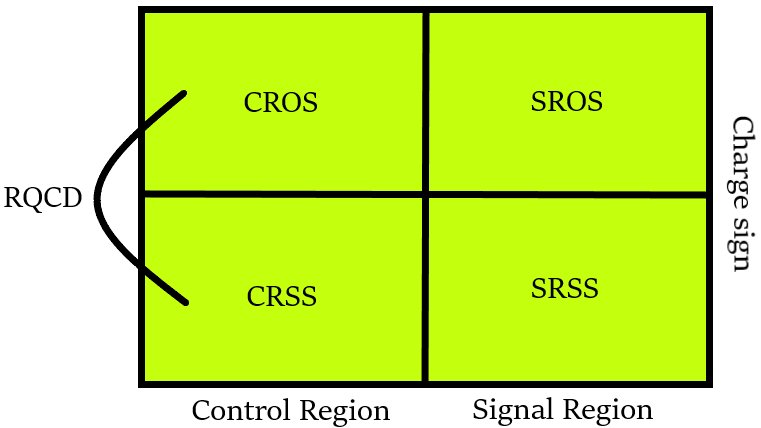
\includegraphics[width=0.5\textwidth]{figures/Fig7.png}
	\caption{Regions defined to estimate MJ background contribution in the SROS region. This data-driven method is also known as the ABCD method.}
	\label{Fig7}
\end{figure}
Table \ref{tab:MJ} summarises inputs into the calculation of the MJ background in the three candidate event samples. 

\begin{table}[]
	\resizebox{\textwidth}{!}{%
		\begin{tabular}{ccccc}
			\rowcolor[HTML]{C0C0C0} 
			\textbf{Sample} & \multicolumn{2}{c}{\cellcolor[HTML]{C0C0C0}\textbf{$\mu \tauhad$}} & \multicolumn{2}{c}{\cellcolor[HTML]{C0C0C0}\textbf{$e \tauhad$}} \\
			& 1-prong                                  & 3-prong                                 & 1-prong                                 & 3-prong                                \\ \hline
			CR OS Data      & 476.0 $\pm$ 22                                 & 270.0 $\pm$ 16                               & 62.0  $\pm$ 8                               & 39.0 $\pm$ 6                               \\
			MC              & 28.608 $\pm$ 4.068                               & 10.531 $\pm$ 1.833                              & 21.058 $\pm$ 10.808                              &              4.794 $\pm$ 1.558                 \\
			CR SS Data      & 366.0 $\pm$ 19                                 & 151.0 $\pm$ 12                                 & 56.0 $\pm$ 7                                & 28.0 $\pm$ 5                                \\
			MC              & 3.46 $\pm$  0.740                               & 0.381 $\pm$ 0.229                                 & 1.152 $\pm$ 0.458 0.444                               &                    0.843 $\pm$             \\ \hline
			RQCD            & 1.234 $\pm$ 0.081                                  & 1.723 $\pm$ 0.178                                 & 0.746 $\pm$ 0.208                                  & 1.260 $\pm$ 0.342                                \\ \hline
			SR SS Data      & 95.0 $\pm$ 10                                  & 13.0 $\pm$ 4                                  & 113.0 $\pm$ 11                                 & 18.0 $\pm$ 4                                 \\
			MC              & 57.257 $\pm$ 4.799                                & 6.761 $\pm$ 2.363                                  & 63.585 $\pm$ 4.793                               & 19.240 $\pm$ 2.651                               \\ \hline
			MJ Background   & 46.577 $\pm$  13.825	                               & 10.748 $\pm$ 13.870                                & 36.887 $\pm$  15.695                              & 0.0 $\pm$ 15.695                                 
		\end{tabular}%
	\caption{Inputs for the calculation of the central value of the MJBG yield in the two final states, $Z\to\mu\tauhad$ and $Z\to e\tauhad$.
		The numbers of data events in the CR OS and CR SS samples are given, together with the total numbers of events in these
		categories expected from simulation.
		The excess of data with respect to simulation is assumed to arise from MJBG and it is used to calculate the value of RQCD.
	}

	\label{tab:MJ}
}





\end{table}

Fig. \ref{Fig12} shows the jetRNN score distributions for the events in the CRs. It can be seen that the samples are dominated by non-simulated background. Fig. shows the jetRNN distribution in the SRSS for the $Z\to\tauhad\mu$ final state.

\begin{figure}[htbp]
	\centering
	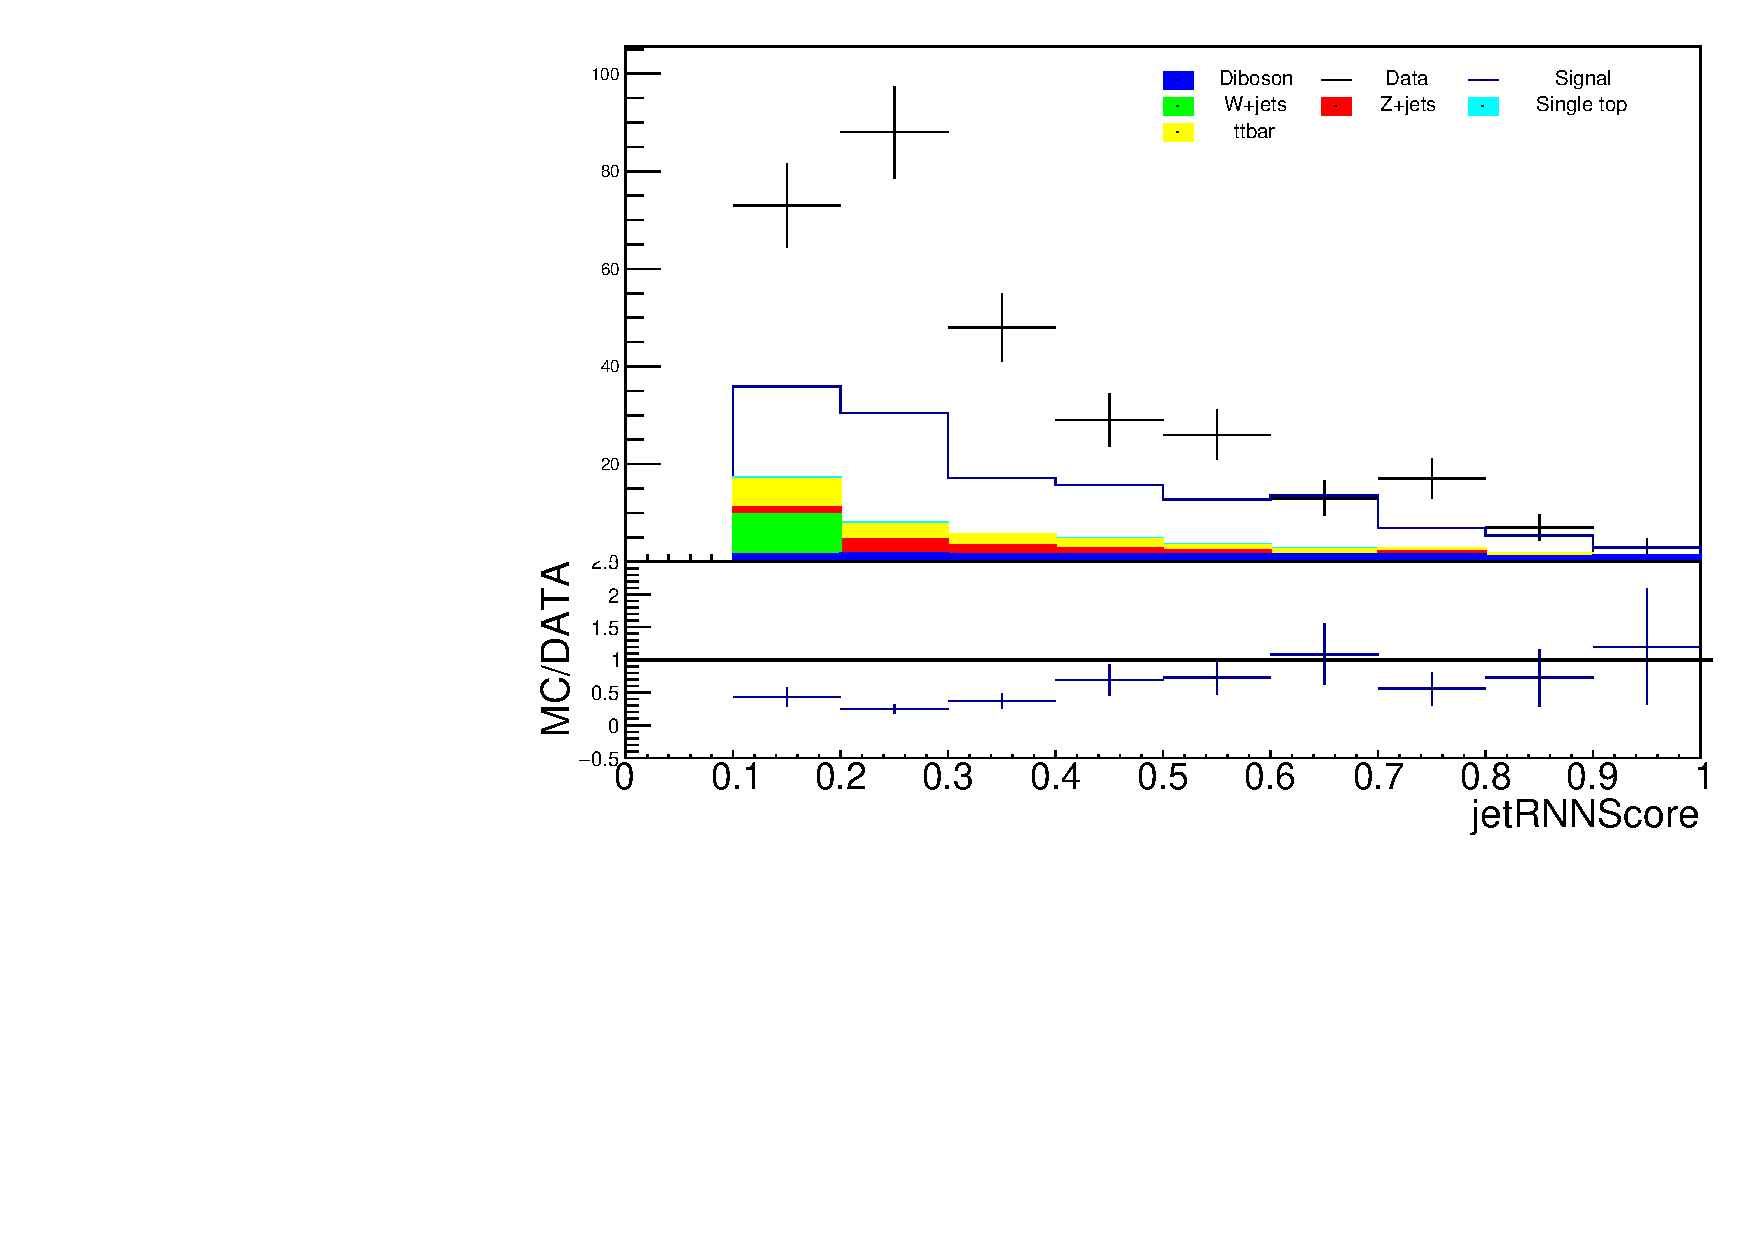
\includegraphics[width=0.5\textwidth]{figures/Fig21}
	\caption{jetRNNScore distribution for 1-prong taus in the SRSS. The data to MC difference gives the shape for the MJBG contribution. After that, the shape is scaled by RQCD to obtain the MJ in the SROS.}
	\label{Fig21}
\end{figure}

\begin{figure}[htbp]
	\centering
	\subfloat[]{\label{Fig12a}{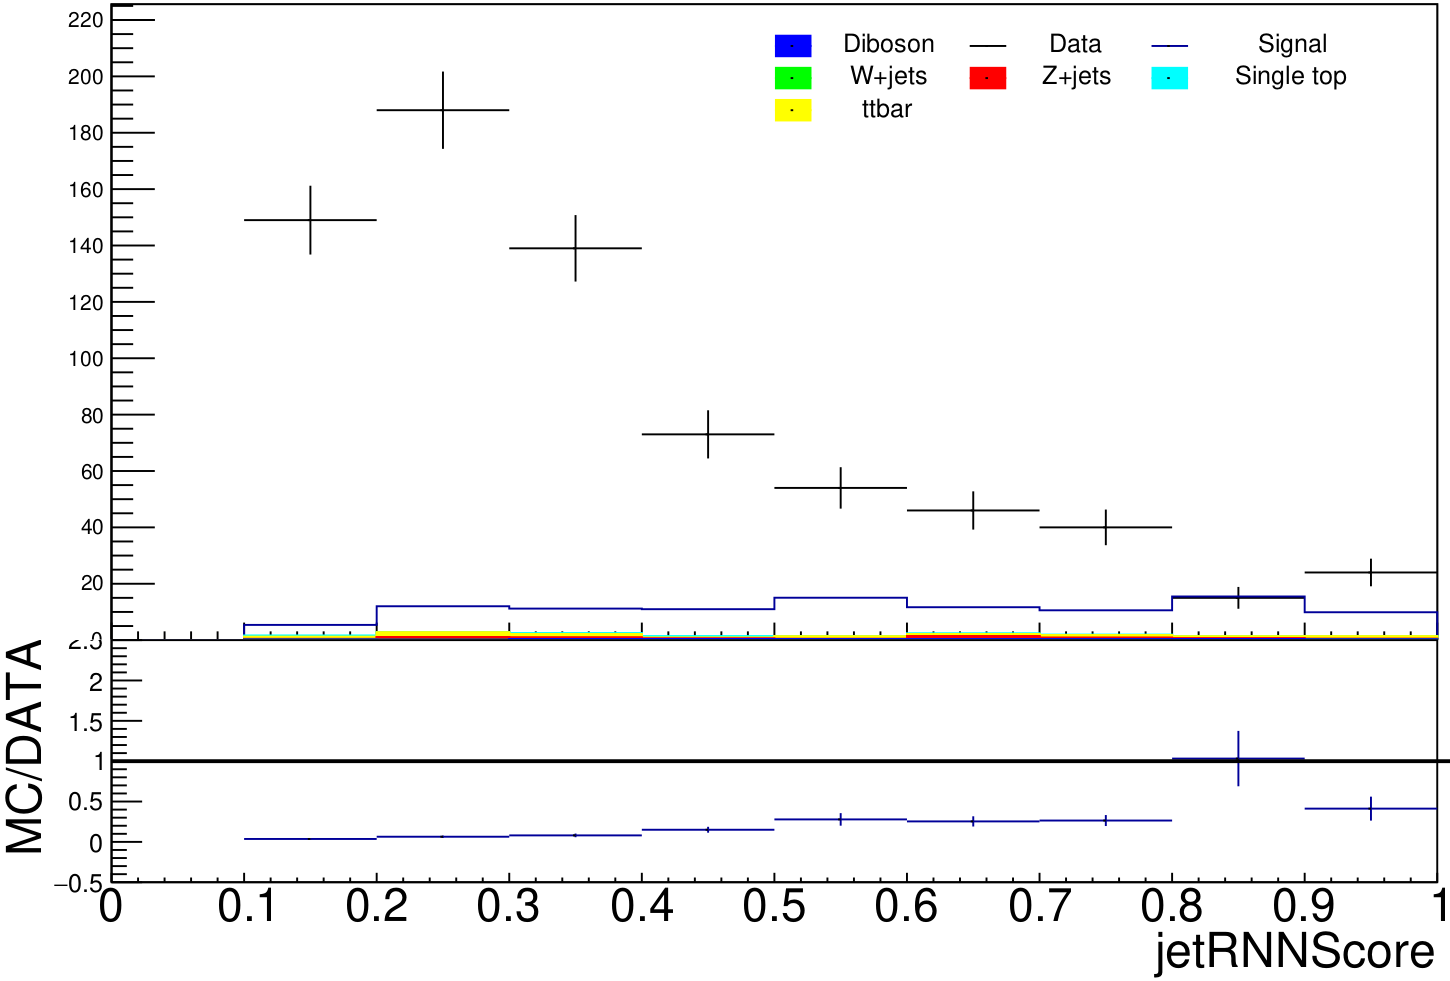
\includegraphics[width=0.50\textwidth]{figures/Fig12a.png}}}
	\subfloat[]{\label{Fig12b}{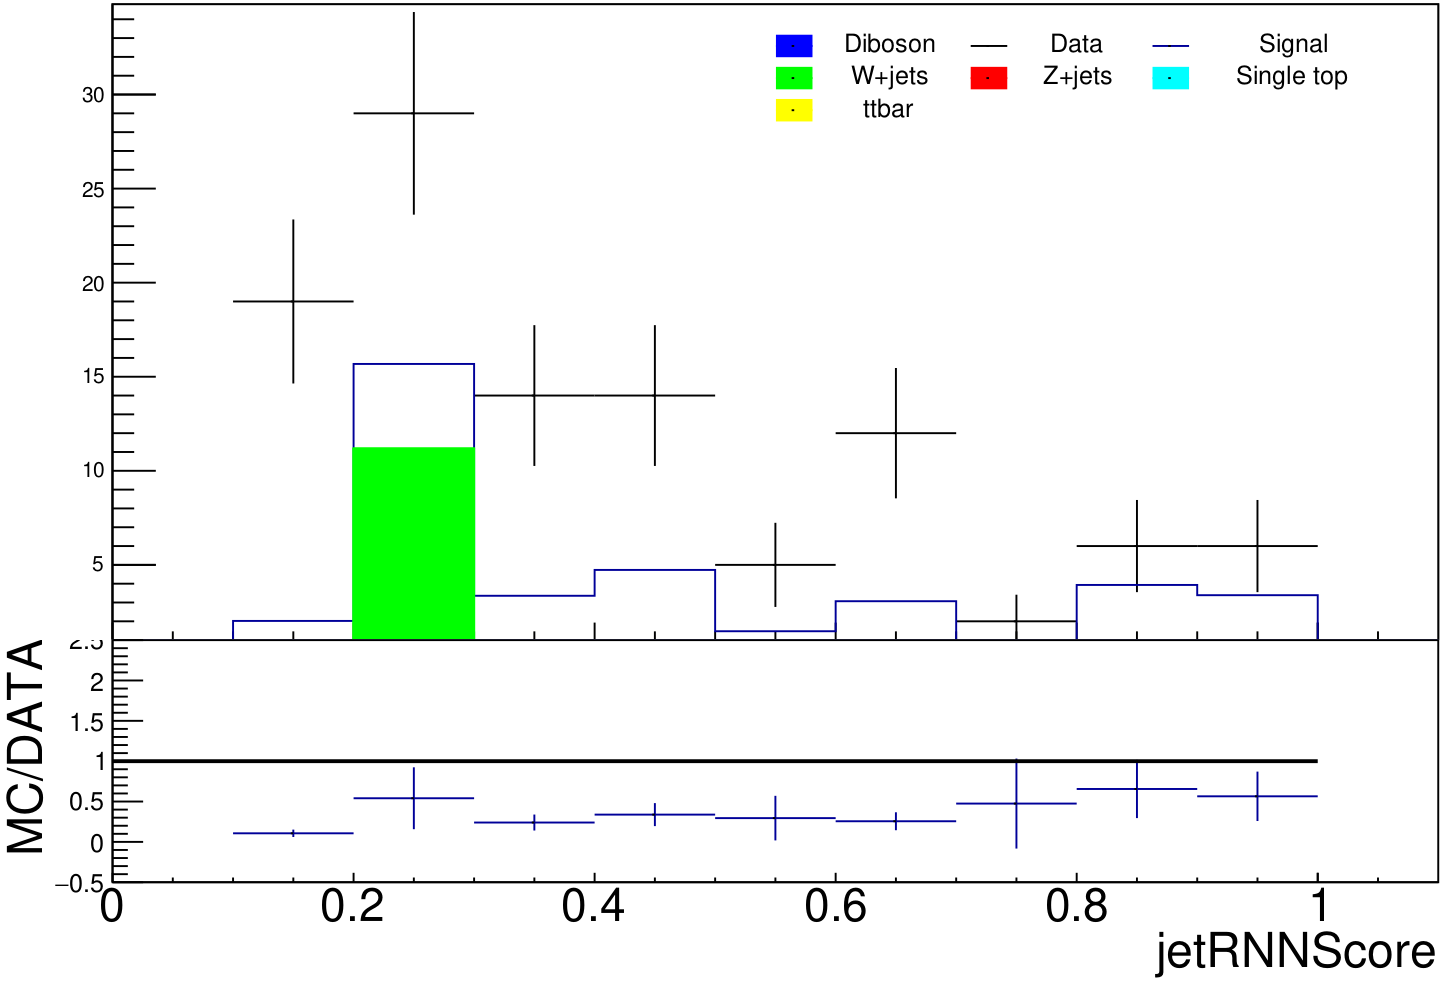
\includegraphics[width=0.50\textwidth]{figures/Fig12b.png}}}\hfill
	\subfloat[]{\label{Fig12c}{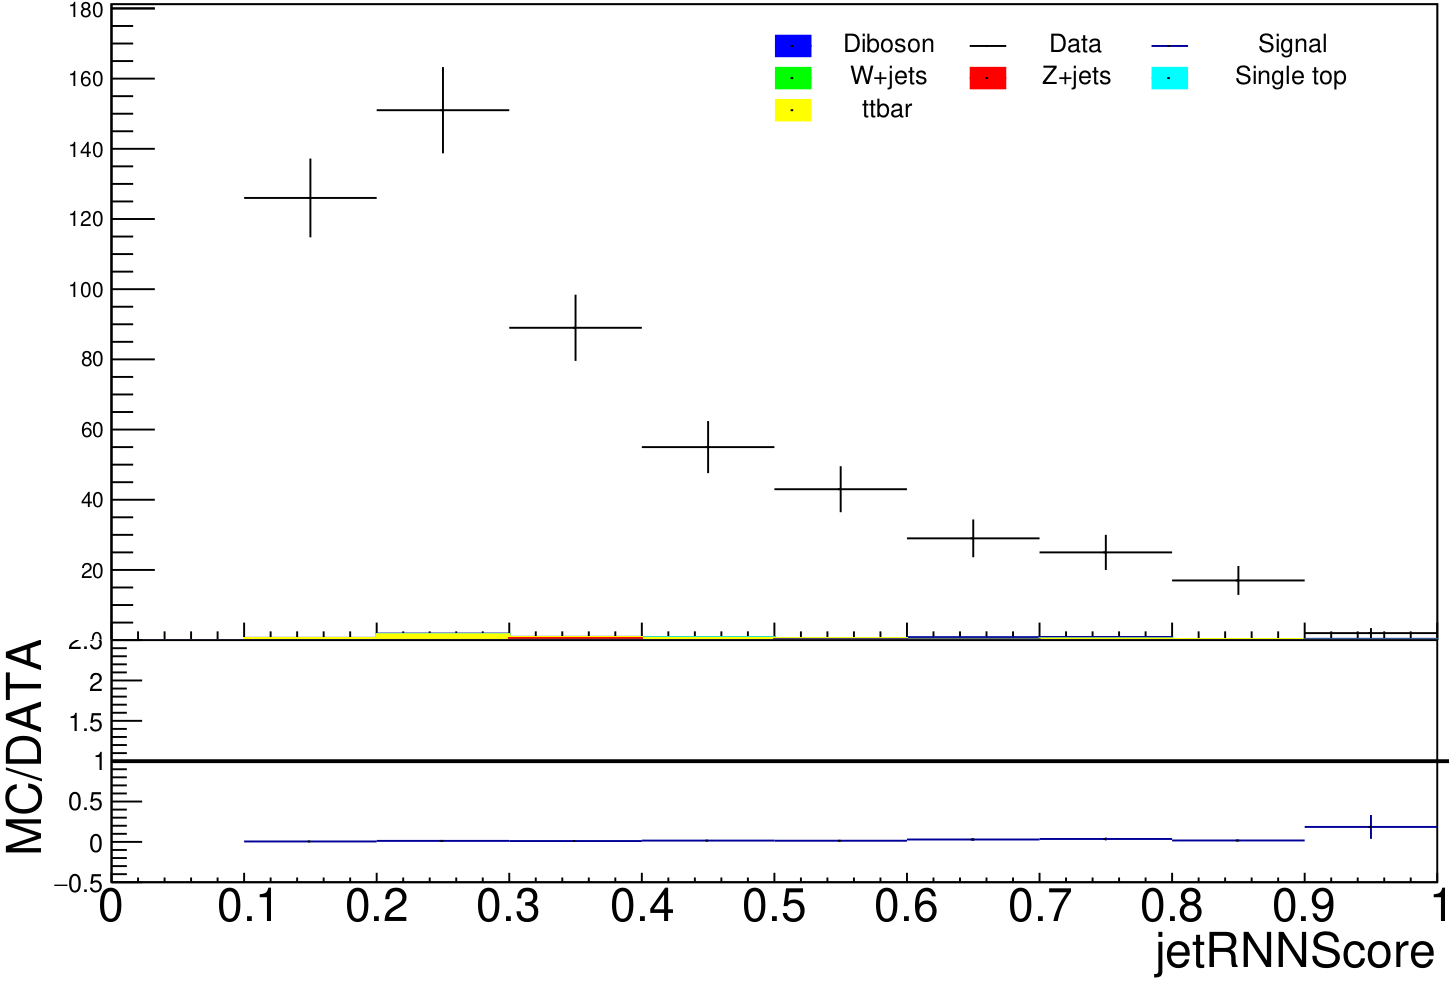
\includegraphics[width=0.50\textwidth]{figures/Fig12c.png}}}
	\subfloat[]{\label{Fig12d}{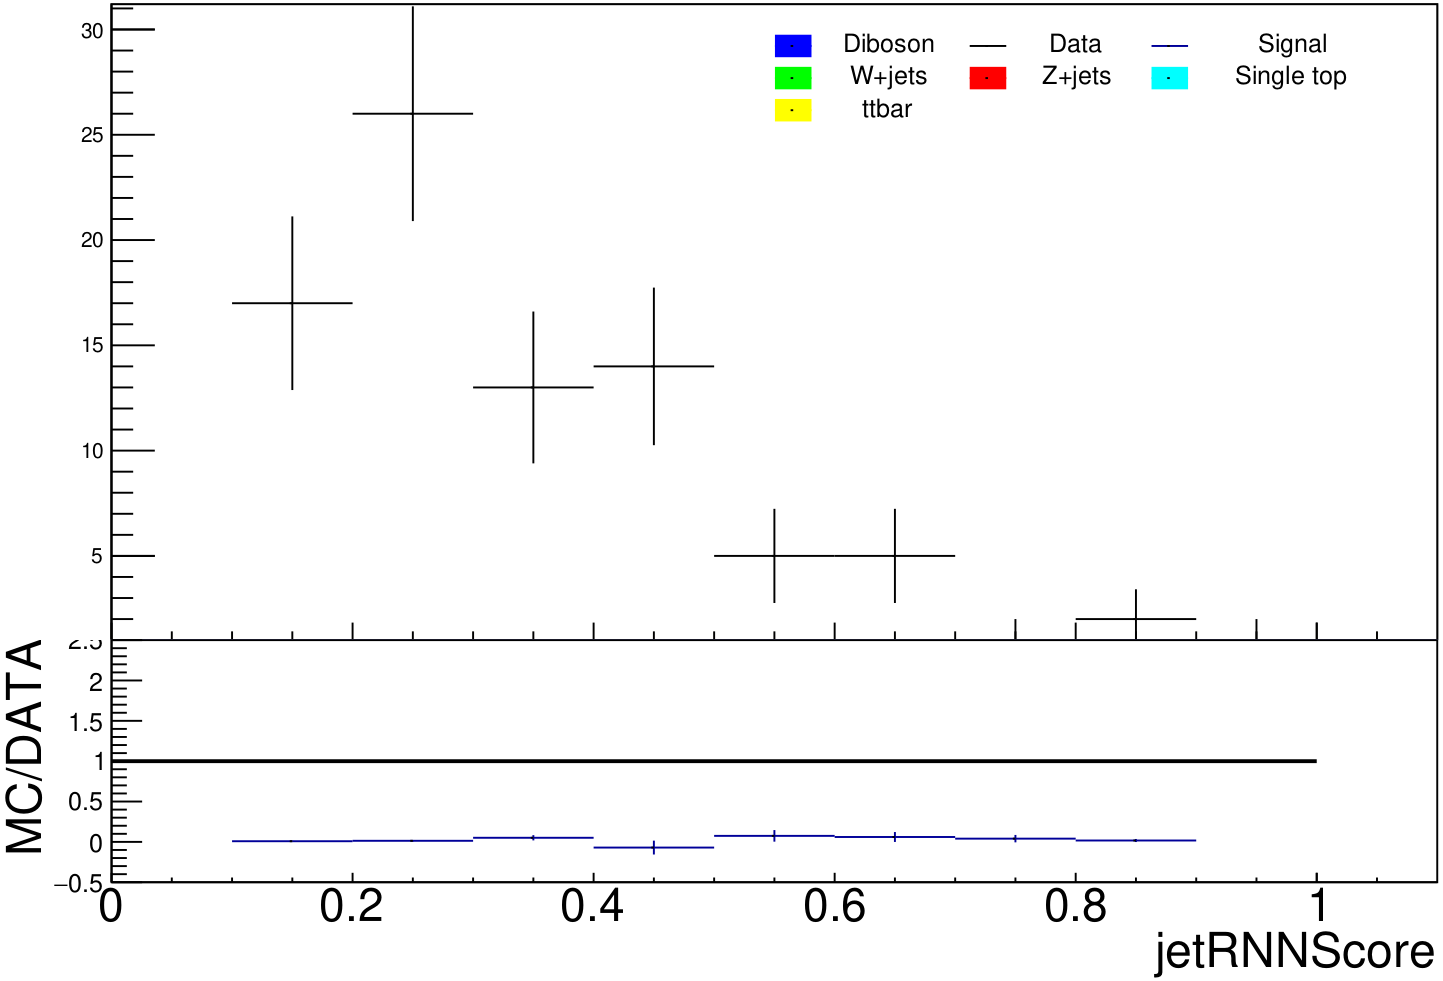
\includegraphics[width=0.50\textwidth]{figures/Fig12d.png}}}
	\caption{Left column (a,c) represents $Z\to\tauhad\mu$ and $Z\to\tauhad e$ is in the right column (b,d). The two figures on top show the CROS and the bottom ones represent the CRSS. All of the plots show the jetRNNScore for 1 prongs. In this case the events used to calculate RQCD are the ones with jetRNNScore$<0.4$.  }
	\label{Fig12}
\end{figure}

\subsection{Electroweak Background}
The electroweak background (EWBG) sources considered are $t\bar{t}$, $\Zjets$, Diboson and single top processes. For all of them, simulated samples are available and they are listed in Table \ref{Table3}. At an early stage of our analysis the $\Wjets$  simulation was checked for correctly accounting for the expected EWBG. This study is described in Appendix \ref{wjetsstudy}. Nonetheless, the final $\Wjets$ contribution to our background yield is so small that an updated study will not improve the quality and precision of our results.  
%-------------------------------------------------------------------------------

%-------------------------------------------------------------------------------
\section{Systematic Uncertainties}\label{Sys}
\label{sec:syst}
%-------------------------------------------------------------------------------

Syst. Uncertainties here.


%-------------------------------------------------------------------------------
\section{Results}\label{Results}
\label{sec:results}
%-------------------------------------------------------------------------------

SFs 1-prong.

\begin{table}[H]
\resizebox{\textwidth}{!}{%
\centering
\begin{tabular}{|c|c|c|c|} 
\hline
\rowcolor[rgb]{0.753,0.753,0.753} Sample (1-prong)                  & Sherpa                                                                 & PoPy-RW                                                                & PoPy                                                                    \\ 
\hline
\rowcolor[rgb]{0.937,0.937,0.937} $p_T$ Range (GeV)                 & \multicolumn{3}{c|}{$p_T>$70}                                                                                                                                                                                             \\ 
\hline
\rowcolor[rgb]{0.604,1,0.6} $C(Z\to\mu\mu)$                         & \textbf{$1.083\pm0.002\pm0.004=0.004$} & \textbf{$0.987\pm0.001\pm0.001=0.002$} & \textbf{$1.182\pm0.002\pm0.001=0.002$}  \\ 
\hline
\rowcolor[rgb]{0.604,1,0.6} $C(Z\to ee)$                            & \textbf{$1.076\pm0.002\pm0.003=0.003$} & \textbf{$1.021\pm0.002\pm0.001=0.002$} & \textbf{$1.227\pm0.002\pm0.001=0.002$}  \\ 
\hline
\rowcolor[rgb]{0.937,0.937,0.937} $p_T$ Range (GeV)                 & \multicolumn{3}{c|}{$p_T>$45}                                                                                                                                                                                             \\ 
\hline
\rowcolor[rgb]{0.588,1,0.984} $C_{\text{Tight-ID}}(Z\to\tau\mu)$    & \textbf{$1.044\pm0.011\pm0.018=0.021$} & \textbf{$0.947\pm0.01\pm0.014=0.017$}  & \textbf{$1.11\pm0.012\pm0.017=0.02$}    \\ 
\hline
\rowcolor[rgb]{0.588,1,0.984} SF\_Tight-ID                          & \textbf{$0.964\pm0.01\pm0.017=0.02$}   & \textbf{$0.959\pm0.01\pm0.014=0.017$}  & \textbf{$0.939\pm0.01\pm0.014=0.017$}   \\ 
\hline
\rowcolor[rgb]{0.992,0.408,0.392} $C_{\text{Tight-ID}}(Z\to\tau e)$ & \textbf{$1.041\pm0.012\pm0.021=0.025$} & \textbf{$0.971\pm0.011\pm0.018=0.022$} & \textbf{$1.138\pm0.014\pm0.023=0.027$}  \\ 
\hline
\rowcolor[rgb]{0.992,0.408,0.392} SF\_Tight-ID                      & \textbf{$0.968\pm0.012\pm0.02=0.023$}  & \textbf{$0.952\pm0.011\pm0.018=0.021$} & \textbf{$0.927\pm0.011\pm0.019=0.022$}  \\ 
\hline
\multicolumn{4}{|c|}{Statistical uncertainty is reported as Correlated $\pm$ Uncorrelated $=$ Total}                                                                                                                                                                                            \\
\hline
\end{tabular}
}
\end{table}


SFs 3-prong.


\begin{table}[H]
	\resizebox{\textwidth}{!}{%
		\centering
		\begin{tabular}{|c|c|c|c|} 
			\hline
			\rowcolor[rgb]{0.753,0.753,0.753} Sample (3-prong)                  & Sherpa                                                                 & PoPy-RW                                                                & PoPy                                                                    \\ 
			\hline
			\rowcolor[rgb]{0.937,0.937,0.937} $p_T$ Range (GeV)                 & \multicolumn{3}{c|}{$p_T>$45}                                                                                                                                                                                             \\ 
			\hline
			\rowcolor[rgb]{0.588,1,0.984} $C_{\text{Tight-ID}}(Z\to\tau\mu)$    & \textbf{$0.924\pm0.019\pm0.038=0.042$} & \textbf{$0.912\pm0.018\pm0.029=0.034$} & \textbf{$1.065\pm0.021\pm0.036=0.041$}  \\ 
			\hline
			\rowcolor[rgb]{0.588,1,0.984} SF\_Tight-ID                          & \textbf{$0.854\pm0.017\pm0.035=0.039$} & \textbf{$0.925\pm0.018\pm0.029=0.034$} & \textbf{$0.901\pm0.018\pm0.03=0.035$}   \\ 
			\hline
			\rowcolor[rgb]{0.992,0.408,0.392} $C_{\text{Tight-ID}}(Z\to\tau e)$ & \textbf{$0.993\pm0.022\pm0.052=0.057$} & \textbf{$0.872\pm0.02\pm0.039=0.044$}  & \textbf{$1.02\pm0.023\pm0.052=0.057$}   \\ 
			\hline
			\rowcolor[rgb]{0.992,0.408,0.392} SF\_Tight-ID                      & \textbf{$0.923\pm0.02\pm0.049=0.053$}  & \textbf{$0.855\pm0.019\pm0.038=0.043$} & \textbf{$0.831\pm0.019\pm0.043=0.047$}  \\ 
			\hline
			\multicolumn{4}{|c|}{Statistical uncertainty is reported as Correlated $\pm$ Uncorrelated $=$ Total}                                                                                                                                                                                            \\
			\hline
		\end{tabular}
	}
\end{table}

% All figures and tables should appear before the summary and conclusion.
% The package placeins provides the macro \FloatBarrier to achieve this.
% \FloatBarrier


%-------------------------------------------------------------------------------
\section{Conclusion}\label{Conclusion}
\label{sec:conclusion}
%-------------------------------------------------------------------------------

Place your conclusion here.


%-------------------------------------------------------------------------------
% If you use biblatex and either biber or bibtex to process the bibliography
% just say \printbibliography here
\printbibliography
% If you want to use the traditional BibTeX you need to use the syntax below.
% \bibliographystyle{obsolete/bst/atlasBibStyleWithTitle}
% \bibliography{QTDiego,bib/ATLAS,bib/CMS,bib/ConfNotes,bib/PubNotes}
%-------------------------------------------------------------------------------

%-------------------------------------------------------------------------------
% Print the list of contributors to the analysis
% The argument gives the fraction of the text width used for the names
%-------------------------------------------------------------------------------
\clearpage
The supporting notes for the analysis should also contain a list of contributors.
This information should usually be included in \texttt{mydocument-metadata.tex}.
The list should be printed either here or before the Table of Contents.
\PrintAtlasContribute{0.30}


%-------------------------------------------------------------------------------
\clearpage
\appendix
\part*{Appendices}
\addcontentsline{toc}{part}{Appendices}
%-------------------------------------------------------------------------------

In an ATLAS note, use the appendices to include all the technical details of your work
that are relevant for the ATLAS Collaboration only (e.g.\ dataset details, software release used).
This information should be printed after the Bibliography.

\end{document}
